\documentclass[11pt,a4paper]{article}
\usepackage{fontspec}
\usepackage{xeCJK}
\setCJKmainfont{STSong}
\setCJKsansfont{STHeiti}
\usepackage{amsmath,amssymb,amsthm}
\usepackage{mathtools}
\usepackage{bm}
\usepackage{booktabs}
\usepackage{array}
\usepackage{enumitem}
\usepackage{geometry}
\usepackage{xcolor}
\usepackage{tcolorbox}
\usepackage{algorithm}
\usepackage{algpseudocode}
\usepackage{pifont}
\usepackage{tikz}
\usetikzlibrary{arrows.meta,positioning,calc,fit,decorations.pathreplacing}
\usepackage[pdfencoding=auto,psdextra]{hyperref}

\geometry{margin=2.5cm}

\newcommand{\loss}{\mathcal{L}}
\newcommand{\E}{\mathbb{E}}
\newcommand{\R}{\mathbb{R}}
\newcommand{\KL}{\mathrm{KL}}
\newcommand{\N}{\mathcal{N}}
\newcommand{\adv}{\mathcal{A}}
\newcommand{\reward}{R}
\newcommand{\softmax}{\mathrm{softmax}}
\newcommand{\sg}{\mathrm{sg}}
\newcommand{\MoF}{\mathrm{MoF}}

\theoremstyle{definition}
\newtheorem{definition}{Definition}
\newtheorem{remark}{Remark}
\newtheorem{proposition}{Proposition}
\newtheorem{corollary}{Corollary}
\newtheorem{lemma}{Lemma}
\newtheorem{theorem}{Theorem}

\title{\textbf{MoF 二阶段训练流水线}\\[0.3em]
\large Stage 1: NFT 路由器训练 \quad $\to$ \quad Stage 2: 学生模型在线蒸馏\\[0.4em]
\large 从 motivation 到算法实现的完整推导}
\author{Flow Factory}
\date{}

\begin{document}
\maketitle

\begin{abstract}
本文系统阐述 MoF (Mixture-of-Flow) 的二阶段训练流水线：
\textbf{Stage 1} (\texttt{trainers/mof/nft.py}) 通过 DiffusionNFT
在 reward 空间中优化 per-set、per-timestep、per-prompt 的 teacher 混合权重；
\textbf{Stage 2} (\texttt{trainers/mof/distill.py}) 把 Stage 1 学到的
\emph{router-induced teacher}（一个动态加权的 teacher 集成）通过 on-policy
轨迹 MSE 蒸馏到一个独立的 student LoRA。我们给出 motivation、形式化定义、
两阶段各自的损失/梯度推导、与代码一一对应的算法伪代码、关键的数值正确性
不变量（autocast cache 与 DDP 权重交换冲突）以及完整的端到端流程图。
全文与 \texttt{trainers/mof/\{nft.py, distill.py, common.py\}} 中的实现严格对齐。
\end{abstract}

\tableofcontents
\newpage

%% ============================================================
\section{Motivation}
\label{sec:motivation}
%% ============================================================

\subsection{背景：单阶段方法的局限}

我们已有 $K$ 个针对不同 reward objective 微调的 LoRA teacher
$\{v^{(k)}\}_{k=1}^K$（如 GenEval / PickScore / OCR），
以及一组对应的 reward function $\{R_j\}$ 和按 source 划分的 prompt 集合
$\{\mathcal{P}_s\}_{s=1}^S$。两条传统路线如下：

\begin{itemize}[leftmargin=1.5em]
\item \textbf{OPD-Average / PCGrad}：把所有 teacher 蒸馏到一个 student。
最优 student velocity 为 teacher velocity 的（投影后）均值，由 Jensen
不等式必然在 in-domain 上退化（\texttt{mof\_gradient\_analysis.tex}
Proposition~3）。
\item \textbf{OPD-Route by source}：student 在每个 source 上拟合对应的
in-domain teacher。等价于分别训练 $K$ 个 student，OOD 泛化能力差。
\end{itemize}

两者的共同问题：student 的 velocity 在每个 $(x, t)$ 点上被 teacher
velocity 的几何关系直接锁定，\textbf{无法利用 trajectory 级的 reward
信号在不同 timestep 偏向不同 teacher}。

\subsection{MoF 的解决思路}

MoF 把搜索空间从 $\R^P$（model weights，$P \sim 10^7$--$10^9$）压缩到
$\R^{K \times T \times S}$（mixing logits，$\sim 10^2$），并直接在
\textbf{reward 空间}中优化 per-timestep 的 teacher 混合权重：
\begin{equation}
v_\lambda(x, t_i, p) = \sum_{k=1}^K \lambda_{k,i,s(p)}\,v^{(k)}(x, t_i, p),
\qquad \sum_k \lambda_{k,i,s} = 1,\;\lambda_{k,i,s} \geq 0
\label{eq:mof_velocity_intro}
\end{equation}

\textbf{时间互补性}（temporal complementarity）允许 $v_\lambda$
\textbf{严格超越任何单一 teacher}：早期 timestep 用擅长 layout 的 teacher，
晚期 timestep 用擅长 aesthetics 的 teacher，最终 reward 综合优于任意
固定选择（详见 \texttt{mof\_gradient\_analysis.tex} Theorem~2）。

\subsection{为什么需要二阶段？}

只有 Stage 1 训练完之后，部署期的推理代价仍然沉重：每个 denoising step
要跑 \textbf{$K$ 次 teacher forward}（甚至包括 router 网络），相比单 LoRA
推理是 $K\times$ 开销。这在生产环境不可接受。

二阶段训练的目的：\textbf{把 Stage 1 学到的"动态加权 teacher 集成"固化
进一个单独的 student LoRA}。

\begin{tcolorbox}[colback=blue!5,colframe=blue!50!black,title=\textbf{二阶段流水线核心思想}]
\begin{center}
\renewcommand{\arraystretch}{1.4}
\begin{tabular}{rcl}
Stage 1 & : & 在 reward 空间中找出最优混合策略 $\psi^*$\\
        &   & \quad （只训练 $\sim 10^2$--$10^6$ 个 mixing 参数）\\[0.2em]
$\downarrow$ & & 把 $\psi^*$ 看作一个"虚拟 teacher" $v^{\MoF^*}$\\[0.2em]
Stage 2 & : & 用 OPD 把 $v^{\MoF^*}$ 蒸馏到 student LoRA\\
        &   & \quad （student 一次 forward 替代 $K$ 次 teacher forward）
\end{tabular}
\end{center}
\end{tcolorbox}

二阶段的优势：

\begin{enumerate}[leftmargin=1.5em]
\item \textbf{推理简化}：部署时单次 student forward 替代 $K$ 次 teacher
  forward + 1 次 router forward。
\item \textbf{Ensemble 收益固化}：把动态混合的 reward 增益编码进单一模型，
  Stage 1 的 reward improvement 通过 distillation 转移到 student。
\item \textbf{绕过 MoF 梯度消失}：Stage 2 在 model-weight 空间训练，不存在
  normalized-mixing 瓶颈（\texttt{mof\_per\_set\_analysis.tex} 第 13 节）。
\item \textbf{OPD 基础设施复用}：Stage 2 沿用 \texttt{trainers/opd} 的
  loader / forward signature cache 等基础设施，仅替换 target 构造。
\end{enumerate}

%% ============================================================
\section{Notation 与形式化}
\label{sec:notation}
%% ============================================================

\subsection{符号表}

\begin{center}
\renewcommand{\arraystretch}{1.3}
\begin{tabular}{cl}
\toprule
\textbf{符号} & \textbf{含义} \\
\midrule
$K$ & Teacher 数量 \\
$T$ & 推理 timesteps 数量 (\texttt{num\_inference\_steps}) \\
$S$ & Prompt set 数量（由 \texttt{TeacherConfig.sources} 决定） \\
$B$ & Batch size \\
$d$ & Latent 维度 $= C \times H \times W$ \\
$x_0 \in \R^d$ & Clean latent（来自 sampled trajectory 的最后一步） \\
$x_{t_i}$ & 在 timestep $t_i$ 上的 noised / trajectory latent \\
$\sigma_i$ & flow-match noise level at $t_i$, $\sigma_i \in [0, 1]$ \\
$v^{(k)}(x, t, c)$ & Teacher $k$ 的 velocity field（frozen）\\
$\psi$ & Mixing module 参数（LUT 是 logits $\ell$；router 是网络参数）\\
$\lambda_{k,i,s}(\psi)$ & Teacher $k$ 在 timestep $i$、set $s$ 上的混合权重 \\
$\bar{\psi}, \bar{\lambda}$ & EMA shadow（off-policy old policy）\\
$\theta$ & Student LoRA 参数（Stage 2 唯一可训）\\
$v^\theta(x, t, c)$ & Student velocity field \\
$\tau$ & Softmax 温度 \\
$\beta$ & NFT positive/negative 插值系数 \\
$\gamma$ & OOD bonus 系数（默认 0.2） \\
$A_{\max}$ & advantage clip 上界 (\texttt{adv\_clip\_range[1]}) \\
\bottomrule
\end{tabular}
\end{center}

\subsection{两种 Mixing Module}

代码中 \texttt{create\_mixing\_module} 工厂函数支持两种实现，二者输出
统一为 $\mathbf{W} \in \R^{K \times B}$（每列归一化），下游使用方式完全一致。

\paragraph{LUT (\texttt{MoFMixingModule})}
离散查表 $\bm{\Lambda} \in \R^{K \times T \times S}$，按整数索引
$(k, t_{\text{idx}}, s)$ 查表后 softmax 得 $\lambda_{k, t_{\text{idx}}, s}$。
适合 prompt 类别稳定、推理步数固定的场景。

\paragraph{Continuous Router (\texttt{MoFAdaLNRouter} / \texttt{MoFMLPRouter})}
连续函数 $\lambda_k(t, \mathbf{c}) = \softmax(f_\psi(t, \mathbf{c}) / \tau)_k$，
其中 $\mathbf{c}$ 来自 prompt embeddings 的 attention pooling 或直接使用
\texttt{pooled\_prompt\_embeds}。adaLN 变体让 timestep 通过
$(\gamma, \beta)$ 调制 text embedding，符合 DiT conditioning 范式
（PixArt-$\alpha$ / SD3 / Flux）。

本文以下统一记 $\lambda_{k}(t, \mathbf{c}; \psi)$，LUT 是其特例
（$\mathbf{c}$ 退化为 source $s$ 的 one-hot）。

\subsection{组合速度（per-sample, per-set）}

设 batch 中样本 $b$ 来自 source $s_b$，混合速度为
\begin{equation}
\boxed{
v_\lambda^{(b)}(x_b, t_i; \psi)
= \sum_{k=1}^K \lambda_{k,i,s_b}(\psi)\;\sg\!\left(v^{(k)}(x_b, t_i, c_b)\right)
}
\label{eq:per_sample_combined}
\end{equation}
其中 $\sg(\cdot)$ 表示 \texttt{.detach()}——\textbf{teacher velocity 永远
detached，梯度只流过 mixing weights}。这是 Stage 1 的核心约定，对应
\texttt{common.py:\_compute\_teacher\_velocities} 的 \texttt{torch.no\_grad()}
+ \texttt{output.noise\_pred.detach()} 实现。

%% ============================================================
\section{Stage 1: MoF-NFT 路由器训练}
\label{sec:stage1}
%% ============================================================

\subsection{优化目标与可学习参数}

Stage 1 的目标：
\begin{equation}
\psi^* = \arg\max_\psi \E_{p \sim \mathcal{D}}\!\left[
\reward_{\text{composite}}\!\left(\mathrm{ODE}(v_\lambda(\cdot;\psi);\, x_T,\, p)\right)
\right]
\label{eq:stage1_obj}
\end{equation}

\textbf{唯一可训参数}：mixing module $\psi$（LUT 的 logits 或 router 的网络参数）。
Teacher 参数全部 frozen，student LoRA 参数虽然
\texttt{requires\_grad=True}（被 \texttt{use\_named\_parameters} 复用做
weight swap），但因为所有 teacher velocities 都 \texttt{.detach()}，梯度
不会流过 teacher——见 \texttt{common.py:\_init\_optimizer} 注释。

\subsection{Reward $\to$ Advantage Pipeline (Option B)}
\label{subsec:advantage_pipeline}

\texttt{common.py:prepare\_feedback} 实现了三步 advantage 流水线，
对应 \texttt{mof\_per\_set\_analysis.tex} Algorithm~2 (Option B)：

\paragraph{Step 1: Per-reward, per-group 标准化。}
对每个 reward $k \in \{1, \ldots, |\mathcal{R}|\}$ 和每个 group $g$
（共享同一 prompt 的 $K$ 个 sample），独立计算：
\begin{equation}
a_k(x_i) = \frac{R_k(x_i) - \mu_{k,g}}{\max(\sigma_{k,g},\,\epsilon)},
\qquad \text{NaN values skipped (applicable\_sources filtering)}
\label{eq:step1}
\end{equation}

\paragraph{Step 2: Advantage 空间聚合（per-set）。}
对样本 $x_i$（来自 source $s_i$，in-domain reward 记为 $\mathrm{in}(s_i)$）：
\begin{equation}
\adv_{\text{combined}}(x_i)
= a_{\mathrm{in}(s_i)}(x_i)
+ \gamma \cdot \frac{1}{|\mathcal{R}_{\mathrm{ood}}^{(i)}|}
  \sum_{j \in \mathcal{R}_{\mathrm{ood}}^{(i)}} a_j(x_i)
\label{eq:step2}
\end{equation}

\paragraph{Step 3: Global-std 归一化 + clipping。}
\begin{equation}
\sigma_{\text{global}} = \mathrm{std}\!\left(\{\adv_{\text{combined}}(x_i)\}_{i=1}^N\right),
\qquad
\adv_{\text{final}}(x_i)
= \mathrm{clip}\!\left(
\frac{\adv_{\text{combined}}(x_i)}{\max(\sigma_{\text{global}},\,\epsilon)},
\;\text{adv\_clip\_min},\;\text{adv\_clip\_max}
\right)
\label{eq:step3}
\end{equation}

\begin{remark}[为什么在 advantage 空间聚合]
GenEval $\in [0,1]$ 与 PickScore $\in [0.83, 0.95]$ 的 raw scale 差异极大。
Step 1 已经把每个 reward 归一化到 $\sim N(0, 1)$，因此 Step 2 中的 $\gamma$
具有\textbf{尺度无关的语义}：OOD advantage 贡献固定 $\gamma$ 比例的信号
强度。在 raw reward 空间聚合则需要为每对 $(R_i, R_j)$ 单独调系数。
\end{remark}

\subsection{NFT Loss}
\label{subsec:nft_loss}

记 advantage 经 $A_{\max} = \texttt{adv\_clip\_range[1]}$ 归一化后的
"normalized advantage"：
\begin{equation}
r = \mathrm{clamp}\!\left(\frac{\adv_{\text{final}}}{2 A_{\max}} + \frac{1}{2},\;0,\;1\right) \in [0, 1]
\label{eq:r_def}
\end{equation}
其中 $r = 1$ 对应最佳 sample，$r = 0$ 对应最差 sample。

\paragraph{Positive / Negative velocity（关于 $v_{\text{old}}$ 对称）。}
\begin{align}
v_{i,b}^{\text{new}}  &= \sum_k \lambda_{k,i,s_b}(\psi)\;\sg(v^{(k)}_{i,b}) \quad\text{（current $\psi$）}
\label{eq:v_new}\\
v_{i,b}^{\text{old}}  &= \sum_k \lambda_{k,i,s_b}(\bar\psi)\;\sg(v^{(k)}_{i,b}) \quad\text{（EMA $\bar\psi$, detached）}
\label{eq:v_old}\\
v_{i,b}^{+}           &= \beta\,v_{i,b}^{\text{new}} + (1-\beta)\,v_{i,b}^{\text{old}}
\label{eq:v_plus}\\
v_{i,b}^{-}           &= (1+\beta)\,v_{i,b}^{\text{old}} - \beta\,v_{i,b}^{\text{new}}
\label{eq:v_minus}
\end{align}

\paragraph{Self-normalized MSE on $x_0$ reconstruction.}
对每个 sample $b$ 和 timestep $i$，flow-matching 噪声化：
\begin{equation}
x_{t_i, b} = (1 - \sigma_i)\,x_{0,b} + \sigma_i\,\varepsilon,
\qquad \varepsilon \sim \N(0, I)
\label{eq:flow_match_noise}
\end{equation}
（\textbf{重要}：$x_{0,b}$ 是 sampled trajectory 的\emph{最后一步} clean
latent；噪声 $\varepsilon$ 是 \emph{每次 optimize 重新采样}的，不来自
sampling 阶段。这与 Stage 2 的 on-policy trajectory 用法不同，见
\S\ref{sec:stage2}。）

预测的 $x_0$：
\begin{equation}
\hat{x}_{0,b}^{\pm}(v) = x_{t_i, b} - \sigma_i\,v
\label{eq:x0_pred}
\end{equation}

Self-normalized MSE（per-sample 标量）：
\begin{equation}
\boxed{
\mathcal{M}_{i,b}(v) =
\frac{\|\hat{x}_{0,b}(v) - x_{0,b}\|_2^2}
{\sg\!\left(\frac{\|\hat{x}_{0,b}(v) - x_{0,b}\|_1}{d}\right)}
}
\label{eq:self_norm_mse}
\end{equation}
分母是 detached 的 mean absolute error（clip 到 $10^{-5}$），
作为自适应归一化权重——重建误差大时分母大，梯度自动缩小。

\paragraph{NFT 总 loss（per-sample, per-timestep）。}
\begin{equation}
\boxed{
\loss_{i,b}^{\text{NFT}}(\psi)
= \frac{r_b\,\mathcal{M}_{i,b}(v_{i,b}^{+}) + (1 - r_b)\,\mathcal{M}_{i,b}(v_{i,b}^{-})}{\beta}\cdot A_{\max}
}
\label{eq:nft_loss_full}
\end{equation}

最终 batch loss（在 $T$ 个 timestep 上累积；代码中通过
\texttt{accelerator.accumulate} 实现 micro-batching）：
\begin{equation}
\loss^{\text{NFT}}(\psi)
= \frac{1}{B \cdot T}\sum_{b=1}^B \sum_{i=1}^T \loss_{i,b}^{\text{NFT}}(\psi)
\label{eq:nft_total}
\end{equation}

\subsection{$\beta$ 在梯度中精确消去}
\label{subsec:beta_cancels}

\begin{theorem}[$\beta$ Cancellation]
\label{thm:beta_cancel}
$\partial \loss_{i,b}^{\text{NFT}}/\partial v_{i,b}^{\text{new}}$ 与 $\beta$
完全无关；只通过 self-normalization weight $w^{\pm} = \sg(\|\hat{x}_0^{\pm} - x_0\|_1 / d)$
作二阶 magnitude 调制（不影响方向）。
\end{theorem}

证明（链式法则系数）：
\begin{equation}
\frac{\partial v^{+}}{\partial v^{\text{new}}} = \beta,\qquad
\frac{\partial v^{-}}{\partial v^{\text{new}}} = -\beta
\end{equation}
代入：
\begin{equation}
\frac{\partial \loss^{\text{NFT}}}{\partial v^{\text{new}}}
= \frac{A_{\max}}{\beta}\!\left[r\!\cdot\!\frac{\partial \mathcal{M}(v^+)}{\partial v^+}\!\cdot\!\beta
+ (1{-}r)\!\cdot\!\frac{\partial \mathcal{M}(v^-)}{\partial v^-}\!\cdot\!(-\beta)\right]
= A_{\max}\!\left[r\frac{\partial \mathcal{M}^+}{\partial v^+} - (1{-}r)\frac{\partial \mathcal{M}^-}{\partial v^-}\right]
\end{equation}
分子 $\beta$ 与分母 $1/\beta$ 精确对消。详见 \texttt{nft\_beta\_analysis.tex}。

\textbf{实践含义}：调整 \texttt{nft\_beta} $\in \{0.01, 0.1, 1.0\}$ 不会
改变 \texttt{grad\_norm} 的数量级，只改变 loss 的绝对值（scaling）。

\subsection{对 mixing logits 的梯度}

对 LUT 模式 $\psi = \ell \in \R^{K \times T \times S}$（router 模式同理，
增加一个 $\partial \ell / \partial \psi_{\text{router}}$ 因子）：
\begin{equation}
\boxed{
\frac{\partial \loss_{i,b}^{\text{NFT}}}{\partial \ell_{j,i,s_b}}
= \frac{\lambda_{j,i,s_b}}{\tau}\;\mathbf{g}_{i,b}^\top\!\left(v^{(j)}_{i,b} - v_{i,b}^{\text{new}}\right)
}
\label{eq:nft_grad_logit}
\end{equation}
其中 $\mathbf{g}_{i,b} = \partial \loss_{i,b}^{\text{NFT}} / \partial v_{i,b}^{\text{new}}\in \R^d$。

跨 timestep / 跨 set 梯度为零（\textbf{Triple Decoupling}，
\texttt{mof\_per\_set\_analysis.tex} Corollary~1）：
\begin{equation}
\frac{\partial \loss_{i,b}^{\text{NFT}}}{\partial \ell_{j,i',s'}} = 0
\quad\text{当 }i' \neq i \text{ 或 } s' \neq s_b
\end{equation}

\begin{remark}[Mean-subtraction 结构]
公式~\eqref{eq:nft_grad_logit} 中 $(v^{(j)} - v^{\text{new}})$ 项是 softmax
归一化约束 $\sum_k \lambda_k = 1$ 的必然结果（Theorem
\texttt{thm:fundamental\_limit}）。当 teachers 共享同一 base model（LoRA
微调），$v^{(j)} - v^{\text{new}} \approx \delta^{(j)} - \bar\delta$，
量级仅为 base velocity 的 1--5\%——这是 NFT 在 LoRA-shared-base 设定下
梯度量级偏小的根因。详细分析与缓解方案见
\texttt{mof\_per\_set\_analysis.tex} 第 13--14 节。
\end{remark}

\subsection{Off-Policy Old/New 结构（EMA）}

\texttt{sampling\_context()} 在 sampling 阶段使用 EMA 权重 $\bar\psi$
生成 trajectory；\texttt{optimize()} 阶段：
\begin{itemize}[leftmargin=1.5em]
\item \textbf{Phase 1（precompute, no\_grad）}：在 EMA 上下文中计算
  $v^{\text{old}}$，detach 后缓存（每 timestep 一份）。
\item \textbf{Phase 2（gradient）}：用当前 $\psi$ 重新计算 $v^{\text{new}}$，
  与缓存的 $v^{\text{old}}$ 一起喂入 NFT loss。
\end{itemize}
这种"sample with $\bar\psi$, optimize with $\psi$"的拆分使 NFT 成为
off-policy——一份 sample 可被多个 inner epoch 复用，提高数据利用率。

\subsection{算法伪代码：Stage 1 NFT 训练循环}

\begin{algorithm}[H]
\caption{MoF-NFT Optimization (\texttt{trainers/mof/nft.py:optimize})}
\label{alg:nft}
\begin{algorithmic}[1]
\Require Sampled trajectories $\{(\mathbf{x}_b, c_b, s_b, \adv_b)\}_{b=1}^N$ from \textsc{Sample}
\Require Mixing module $\psi$, EMA shadow $\bar\psi$, frozen teachers $\{v^{(k)}\}$
\Require NFT $\beta$, temperature $\tau$, $A_{\max}$, train timesteps $T$
\Statex
\For{inner\_epoch $= 1, \ldots, N_{\text{inner}}$}
  \State shuffle samples
  \For{each micro-batch $\mathcal{B}$ of size $B$}
    \State $x_0 \gets \mathcal{B}.\text{all\_latents}[:, -1]$ \Comment{Final clean latent}
    \State $\{s_b\}_{b=1}^B \gets$ \Call{GetSetIDs}{$\mathcal{B}$}

    \Statex \quad\textcolor{blue}{\textit{// Phase 1: Precompute $v^{\text{old}}$ with EMA $\bar\psi$ (no\_grad)}}
    \State \texttt{adapter.rollout()}
    \State $\{t_i\}_{i=1}^T \gets$ \Call{SampleTimesteps}{$B$} \Comment{logit-normal / uniform / discrete}
    \For{$i = 1, \ldots, T$}
      \State $\sigma_i \gets$ \Call{FlowMatchSigma}{$t_i$}
      \State $\varepsilon_i \sim \N(0, I)$
      \State $x_{t_i} \gets (1 - \sigma_i) x_0 + \sigma_i \varepsilon_i$ \Comment{Eq.~\eqref{eq:flow_match_noise}}
      \State $\{v^{(k)}_i\}_{k=1}^K \gets$ \Call{TeacherForward}{$x_{t_i}, t_i, c$}
        \Comment{See Alg.~\ref{alg:teacher_forward}}
      \State \textbf{with} \texttt{sampling\_context()} (EMA $\bar\psi$):
        $v^{\text{old}}_i \gets \sum_k \lambda_k(t_i, c; \bar\psi) \cdot v^{(k)}_i$
      \State cache $(x_{t_i}, \sigma_i, v^{\text{old}}_i, \{v^{(k)}_i\})$
    \EndFor

    \Statex \quad\textcolor{blue}{\textit{// Phase 2: Compute NFT loss + backward (with grad)}}
    \State \texttt{adapter.train()}
    \For{$i = 1, \ldots, T$}
      \State \textbf{with} \texttt{accelerator.accumulate}($\psi$):
      \State \quad $v^{\text{new}}_i \gets \sum_k \lambda_k(t_i, c; \psi) \cdot \sg(v^{(k)}_i)$
        \Comment{Gradient flows here only}
      \State \quad $\adv \gets \mathrm{clip}(\mathcal{B}.\text{advantage}, -A_{\max}, A_{\max})$
      \State \quad $r \gets \mathrm{clamp}(\adv / (2 A_{\max}) + 0.5,\,0,\,1)$
      \State \quad $v^{+}_i \gets \beta v^{\text{new}}_i + (1-\beta) v^{\text{old}}_i$
      \State \quad $v^{-}_i \gets (1+\beta) v^{\text{old}}_i - \beta v^{\text{new}}_i$
      \State \quad $\loss_i \gets \big(r\,\mathcal{M}_i(v^{+}_i) + (1-r)\,\mathcal{M}_i(v^{-}_i)\big) / \beta \cdot A_{\max}$
        \Comment{Eq.~\eqref{eq:nft_loss_full}}
      \State \quad (optional) $\loss_i \mathrel{+}= \beta_{\text{KL}} \cdot \|v^{\text{new}}_i - v^{\text{ref}}_i\|^2$
      \State \quad \texttt{accelerator.backward}($\loss_i$)
      \If{\texttt{accelerator.sync\_gradients}}
        \State \texttt{clip\_grad\_norm}($\psi$, \texttt{max\_grad\_norm})
        \State \texttt{optimizer.step()}; \texttt{optimizer.zero\_grad()}
      \EndIf
    \EndFor
  \EndFor
\EndFor
\State $\bar\psi \gets$ \Call{EMAStep}{$\psi, \bar\psi$, decay} \Comment{End-of-epoch EMA update}
\end{algorithmic}
\end{algorithm}

\subsection{Sampling 阶段}

NFT sampling 与 GRPO 不同，\textbf{不需要 log-probability}：
\texttt{nft.py:\_build\_sample\_kwargs} 设置 \texttt{compute\_log\_prob=False}
和 \texttt{trajectory\_indices=[-1]}（只保留最后一步 clean latent，节省内存）。

\begin{algorithm}[H]
\caption{MoF Sampling Phase (\texttt{common.py:sample})}
\label{alg:sample}
\begin{algorithmic}[1]
\Require Per-source dataloaders, EMA $\bar\psi$
\Statex
\State \texttt{adapter.rollout()}
\For{batch in \Call{InterleavedSourceIter}{}} \Comment{round-robin per-source}
  \State $s \gets$ \Call{GetBatchSetID}{batch}
  \State \textbf{with} \texttt{\_mof\_inference\_context}($s$):
  \Comment{Patches \texttt{adapter.forward} to $\sum_k \lambda_k v^{(k)}$}
  \State \quad sample\_kwargs $\gets$ \Call{BuildSampleKwargs}{batch}
        \Comment{NFT: only final latent}
  \State \quad samples $\gets$ \texttt{adapter.inference}(**sample\_kwargs)
  \State stitch metadata (\texttt{\_\_source\_\_}, \texttt{include}, \ldots)
        $\to$ \texttt{sample.extra\_kwargs}
\EndFor
\State Compute rewards on all samples; run advantage pipeline (Eqs.~\eqref{eq:step1}--\eqref{eq:step3})
\State \Return samples (each carries \texttt{advantage} field)
\end{algorithmic}
\end{algorithm}

\subsection{数值正确性不变量（HARD RULES）}
\label{subsec:invariants}

下面两条不变量是 \texttt{CLAUDE.md} 列出的硬性约束，违反会导致
\textbf{所有 teacher 静默产出相同输出}。Stage 1 和 Stage 2 都必须遵守。

\paragraph{不变量 1：Autocast cache 与 weight swap 互斥。}
\texttt{adapter.use\_named\_parameters(name)} 通过
\texttt{.data.copy\_()} 交换权重，保留同一 \texttt{data\_ptr}。autocast
cache 按 \texttt{data\_ptr} 索引 cast 后的 tensor，因此 swap 到
teacher\_1 后仍服务 teacher\_0 的 cached cast——所有 teacher 静默
产出相同输出。

\textbf{对策}：在 weight-swap 循环外侧 disable autocast cache：
\begin{verbatim}
prev = torch.is_autocast_cache_enabled()
torch.set_autocast_cache_enabled(False)
try:
    for name in teacher_names:
        with adapter.use_named_parameters(name):
            output = adapter.forward(...)
finally:
    torch.set_autocast_cache_enabled(prev)
\end{verbatim}

\paragraph{不变量 2：DDP 内部 buffer 与 weight swap 互斥（inference path）。}
DDP 在初始化时构建 gradient bucketing buffers，\texttt{.data.copy\_()}
\textbf{不更新}这些 buffer。在 \texttt{torch.no\_grad()} inference 模式下
调用 DDP-wrapped module，仍然读取 stale buffer。

\textbf{对策}：\texttt{mof/utils.py:bypass\_ddp\_for\_weight\_swap} 在
inference 期间临时把 component 指向 unwrapped module：
\begin{verbatim}
@contextmanager
def bypass_ddp_for_weight_swap(adapter):
    unwrapped = adapter.get_component_unwrapped('transformer')
    wrapped = adapter.get_component('transformer')
    if unwrapped is not wrapped:
        adapter.set_component('transformer', unwrapped)
    try:
        yield
    finally:
        if unwrapped is not wrapped:
            adapter.set_component('transformer', wrapped)
\end{verbatim}

两条不变量在以下三处实施：
\begin{enumerate}[leftmargin=1.5em]
\item \texttt{common.py:\_compute\_teacher\_velocities}（用于 NFT optimize）
\item \texttt{common.py:\_mof\_inference\_context}（用于 sampling）
\item \texttt{distill.py:\_compute\_teacher\_velocities}（用于 distill 的 pre-pass）
\end{enumerate}

\begin{algorithm}[H]
\caption{Safe Teacher Forward (autocast + DDP invariants)}
\label{alg:teacher_forward}
\begin{algorithmic}[1]
\Function{TeacherForward}{$x_{t}$, $t$, $c$}
  \State $\text{prev\_cache} \gets$ \texttt{torch.is\_autocast\_cache\_enabled()}
  \State \texttt{torch.set\_autocast\_cache\_enabled(False)}
  \State \textbf{with} \Call{BypassDDPForWeightSwap}{adapter}, \texttt{torch.no\_grad()}:
  \State \quad velocities $\gets [\,]$
  \State \quad \textbf{for} name $\in$ teacher\_names \textbf{do}
  \State \qquad \textbf{with} \texttt{adapter.use\_named\_parameters}(name):
  \State \qquad\quad out $\gets$ \texttt{adapter.forward}($x_t, t, c$)
  \State \qquad velocities.append(\texttt{out.noise\_pred.detach()})
  \State \texttt{torch.set\_autocast\_cache\_enabled(prev\_cache)}
  \State \Return \texttt{stack(velocities, dim=0)} \Comment{$(K, B, C, H, W)$}
\EndFunction
\end{algorithmic}
\end{algorithm}

%% ============================================================
\section{The Bridge: Router-Induced Teacher}
\label{sec:bridge}
%% ============================================================

Stage 1 收敛后，最优 mixing 参数 $\psi^*$ 定义了一个\textbf{动态加权的
虚拟 teacher}：

\begin{definition}[Router-Induced Teacher]
\label{def:router_teacher}
\begin{equation}
\boxed{
v^{\MoF^*}(x, t, c)
\triangleq \sum_{k=1}^K \lambda_k\!\left(t, c; \psi^*\right) \cdot v^{(k)}(x, t, c)
}
\label{eq:router_teacher}
\end{equation}
\end{definition}

\begin{proposition}[$v^{\MoF^*}$ 是合法的 flow-matching velocity field]
\label{prop:legal_flow}
对任意 $\psi^*$，由于 $\sum_k \lambda_k = 1$, $\lambda_k \geq 0$，
$v^{\MoF^*}$ 是 $K$ 个合法 velocity field 的逐点凸组合，仍满足连续性方程
$\partial_t p_t + \nabla\cdot(p_t v^{\MoF^*}) = 0$ 的离散化形式。
（\texttt{mof\_gradient\_analysis.tex} Proposition~1。）
\end{proposition}

\subsection{为什么蒸馏 $v^{\MoF^*}$ 是合理的}

\begin{enumerate}[leftmargin=1.5em]
\item \textbf{Reward 最优性已保证}：$v^{\MoF^*}$ 在 $\psi^*$ 收敛点上达到
  Stage 1 reward objective~\eqref{eq:stage1_obj} 的局部最优。蒸馏目标是
  \textbf{保持这个 reward 增益}，同时压缩推理代价。

\item \textbf{蒸馏从 RL 退化为监督学习}：Stage 2 不再需要 reward
  evaluation——target $v^{\MoF^*}$ 是 well-defined 的 deterministic
  function。loss 是 vanilla MSE。

\item \textbf{绕过 normalized-mixing 梯度瓶颈}：Stage 1 中 softmax
  mean-subtraction 把梯度限制在 $\delta^{(j)} - \bar\delta$ 量级
  （\texttt{mof\_per\_set\_analysis.tex} Theorem
  \texttt{thm:fundamental\_limit}）；Stage 2 的 student 是
  unconstrained model weight，梯度量级 $\sim O(1)$。

\item \textbf{推理代价摊销}：Stage 1 训练时 $K$ 倍 teacher forward 是
  一次性投资；Stage 2 之后每一次部署推理只需 student 一次 forward。
\end{enumerate}

\subsection{Stage 2 的形式化目标}

\begin{equation}
\theta^* = \arg\min_\theta\; \E_{p, x_T \sim \N(0, I)}\!\left[
\sum_{i=1}^T \Big\| v^\theta(x_{t_i}^\theta, t_i, c) - v^{\MoF^*}(x_{t_i}^\theta, t_i, c) \Big\|_2^2
\right]
\label{eq:stage2_obj}
\end{equation}

其中 $\{x_{t_i}^\theta\}_{i=1}^T$ 是 \textbf{student 自己生成的轨迹}：
\begin{equation}
x_{t_{i+1}}^\theta = \texttt{scheduler.step}(x_{t_i}^\theta,\, v^\theta(x_{t_i}^\theta, t_i, c),\, t_i)
\label{eq:student_traj}
\end{equation}

这正是 OPD (On-Policy Distillation) 的范式：在 student 当前 policy 访问的
state 分布上做 distillation——保证训练分布与部署分布一致。

%% ============================================================
\section{Stage 2: 在线轨迹蒸馏}
\label{sec:stage2}
%% ============================================================

\subsection{Stage 2 vs Stage 1 的根本区别}

\begin{center}
\renewcommand{\arraystretch}{1.5}
\footnotesize
\begin{tabular}{@{}p{3.5cm} p{5cm} p{5cm}@{}}
\toprule
& \textbf{Stage 1 (NFT)} & \textbf{Stage 2 (Distill)} \\
\midrule
可训参数 & Mixing $\psi$ ($\sim 10^2$--$10^6$) & Student LoRA $\theta$ ($\sim 10^7$) \\
Loss 类型 & Reward-weighted self-norm MSE on $x_0$ & Pure MSE on velocity \\
需要 reward? & \ding{51}（驱动 advantage） & \ding{55}（target 由 $\psi^*$ 给出） \\
On/Off-policy & Off-policy (EMA $\bar\psi$ for sampling) & On-policy (student 生成 trajectory) \\
Trajectory 用法 & 仅取最后 $x_0$ 用于 NFT noise resample & 全部 $\{x_{t_i}\}$ 都进入 loss \\
Teacher forward 频率 & 每 inner epoch 每 timestep 一次 & 每 batch 每 timestep 一次（pre-pass） \\
梯度量级瓶颈 & $\|v^{(j)} - \bar{v}\| \sim$ LoRA residual & 无（model weight space） \\
\bottomrule
\end{tabular}
\end{center}

\subsection{Sampling Phase（On-Policy Student Trajectory）}

\texttt{distill.py:sample} 中，student 用\textbf{自己当前的权重} $\theta$
生成完整 denoising trajectory：
\begin{align}
x_T &\sim \N(0, I)\\
\text{for } i &= 0, 1, \ldots, T-1: \\
v^\theta_i &= v^\theta(x_{t_i}, t_i, c) \\
x_{t_{i+1}} &= \texttt{scheduler.step}(x_{t_i}, v^\theta_i, t_i)
\end{align}
所有 $\{x_{t_i}\}_{i=0}^T$ 通过 \texttt{trajectory\_indices} 全部存入
\texttt{batch["all\_latents"]}（\texttt{compute\_trajectory\_indices}
基于 \texttt{train\_timestep\_indices} 选择存储位置）。

\textbf{关键差异}：Stage 2 sampling \emph{不调用 teachers，也不调用
router}——纯粹 student 自演。Teacher / router 只在 optimize 阶段的
pre-pass 中介入。

\subsection{Optimization Phase（2-Pass 模式）}

\texttt{distill.py:optimize} 采用与 \texttt{trainers/opd}
完全相同的 2-pass 设计：

\paragraph{Pre-pass（no\_grad，逐 timestep 缓存 target）。}
\begin{equation}
v^{\text{target}}_{i,b} \gets \sum_{k=1}^K \lambda_k(t_i, c_b; \psi^*) \cdot \sg(v^{(k)}(x_{t_i,b}, t_i, c_b))
\label{eq:target_construction}
\end{equation}
其中 $x_{t_i,b}$ 来自 student trajectory（\texttt{batch["all\_latents"]}），
$\psi^*$ 从 \texttt{mof\_state.pt} checkpoint 加载（\textbf{frozen}）。

Pre-pass 中：
\begin{enumerate}[leftmargin=1.5em]
\item 对每个 training timestep $i$，运行 \textbf{$K$ 次 teacher forward}
  （受 Alg.~\ref{alg:teacher_forward} 保护）；
\item 调用 \texttt{\_get\_mof\_weights} 获得 $\lambda_k$（router 模式：
  \texttt{router(t, prompt\_embeds, pooled)}；LUT 模式：按
  \texttt{timestep\_index} 和 \texttt{\_\_source\_\_} 索引）；
\item 计算 $v^{\text{target}}_i$ 并 \textbf{detach 缓存}。
\end{enumerate}

\paragraph{Main pass（with grad，纯 student forward + MSE）。}
\begin{equation}
\boxed{
\loss_{i,b}^{\text{distill}}(\theta) = \big\|v^\theta(x_{t_i,b}, t_i, c_b) - \sg(v^{\text{target}}_{i,b})\big\|_2^2
}
\label{eq:distill_loss}
\end{equation}

总 loss：
\begin{equation}
\loss^{\text{distill}}(\theta) = \frac{1}{B \cdot T \cdot d}\sum_{b=1}^B \sum_{i=1}^T \loss_{i,b}^{\text{distill}}(\theta)
\label{eq:distill_total}
\end{equation}

代码中是 \texttt{((v\_student.float() - v\_target.float()) ** 2).mean()}，
即在所有维度（包括 $d = C \cdot H \cdot W$）上取平均。

\subsection{为什么必须 2-Pass？}
\label{subsec:why_two_pass}

将 pre-pass 与 main-pass 分离是\textbf{正确性约束}，不是性能优化。原因：

\begin{enumerate}[leftmargin=1.5em]
\item Teacher forward 必须 \texttt{use\_named\_parameters} swap weights；
\item Weight swap 必须搭配 \texttt{torch.no\_grad()} +
  \texttt{bypass\_ddp\_for\_weight\_swap} +
  \texttt{set\_autocast\_cache\_enabled(False)}（不变量
  \S\ref{subsec:invariants}）；
\item 而 \texttt{accelerator.accumulate(student\_module)} 上下文要求：
  \begin{itemize}[leftmargin=1em]
    \item gradient flow 必须经过 wrapped DDP module（不能 bypass DDP）；
    \item autocast cache 必须开启（性能要求）。
  \end{itemize}
\end{enumerate}

把 teacher forward（要求 bypass DDP / no autocast cache）放进
\texttt{accumulate} 上下文（要求 wrapped DDP / autocast cache）会
\textbf{同时触发两条不变量违例}——所有 teacher 静默产出相同输出，蒸馏目标
退化为单一 teacher（甚至是 student 自己）。

2-pass 设计是唯一正确路径：把所有 teacher swap 集中到 pre-pass 内，
缓存 detached target；main-pass 只触碰 student 本身，gradient flow 完全
受 DDP 控制。

\subsection{算法伪代码：Stage 2 蒸馏循环}

\begin{algorithm}[H]
\caption{MoF On-Policy Distillation (\texttt{trainers/mof/distill.py:optimize})}
\label{alg:distill}
\begin{algorithmic}[1]
\Require Student trajectories $\{(\mathbf{x}^\theta, c, s)\}_{b=1}^N$ from \textsc{Sample} (Alg.~\ref{alg:distill_sample})
\Require Frozen mixing $\psi^*$ (loaded from \texttt{mof\_state.pt})
\Require Frozen teachers $\{v^{(k)}\}_{k=1}^K$, train timestep indices $\mathcal{T}$
\Statex
\State \texttt{adapter.train()}
\For{inner\_epoch $= 1, \ldots, N_{\text{inner}}$}
  \State shuffle samples
  \For{each micro-batch $\mathcal{B}$ of size $B$}
    \State $\text{idx\_map} \gets \mathcal{B}.\text{latent\_index\_map}$
    \Statex \quad\textcolor{blue}{\textit{// === Pre-pass: cache $v^{\text{target}}$ (no\_grad) ===}}
    \State $V^{\text{target}} \gets [\,]$
    \For{$\hat{i} \in \mathcal{T}$} \Comment{e.g., $\{0, \ldots, T{-}1\}$ for ODE}
      \State $t_{\hat{i}} \gets \mathcal{B}.\text{timesteps}[:, \hat{i}]$
      \State $x_{t_{\hat{i}}} \gets \mathcal{B}.\text{all\_latents}[:, \text{idx\_map}[\hat{i}]]$
        \Comment{Student-visited point}
      \State forward\_kwargs $\gets$ \Call{BuildForwardKwargs}{$\mathcal{B}, t_{\hat{i}}, x_{t_{\hat{i}}}$}
      \State $\{v^{(k)}_{\hat{i}}\}_{k=1}^K \gets$ \Call{TeacherForward}{forward\_kwargs}
        \Comment{Alg.~\ref{alg:teacher_forward}}
      \State $\mathbf{w}_{\hat{i}} \gets$ \Call{GetMoFWeights}{$t_{\hat{i}}, \mathcal{B}, \hat{i}$}
        \Comment{router or LUT}
      \State $v^{\text{target}}_{\hat{i}} \gets \sum_k \mathbf{w}_{\hat{i}}^{(k)} \cdot v^{(k)}_{\hat{i}}$
        \Comment{Eq.~\eqref{eq:target_construction}}
      \State $V^{\text{target}}.\text{append}(v^{\text{target}}_{\hat{i}}.\text{detach}())$
    \EndFor

    \Statex \quad\textcolor{blue}{\textit{// === Main pass: student forward + MSE (with grad) ===}}
    \For{$\hat{i} \in \mathcal{T}$}
      \State \textbf{with} \texttt{accelerator.accumulate}($\theta$):
      \State \quad $t_{\hat{i}} \gets \mathcal{B}.\text{timesteps}[:, \hat{i}]$
      \State \quad $x_{t_{\hat{i}}} \gets \mathcal{B}.\text{all\_latents}[:, \text{idx\_map}[\hat{i}]]$
      \State \quad forward\_kwargs $\gets$ \Call{BuildForwardKwargs}{$\mathcal{B}, t_{\hat{i}}, x_{t_{\hat{i}}}$}
      \State \quad $v^\theta_{\hat{i}} \gets$ \texttt{adapter.forward}(forward\_kwargs).noise\_pred
      \State \quad $\loss \gets \mathrm{mean}\!\left(\big(v^\theta_{\hat{i}} - V^{\text{target}}_{\hat{i}}\big)^2\right)$
        \Comment{Eq.~\eqref{eq:distill_loss}}
      \State \quad \texttt{accelerator.backward}($\loss$)
      \If{\texttt{accelerator.sync\_gradients}}
        \State \texttt{clip\_grad\_norm}($\theta$, \texttt{max\_grad\_norm})
        \State \texttt{optimizer.step()}; \texttt{optimizer.zero\_grad()}
      \EndIf
    \EndFor
  \EndFor
\EndFor
\end{algorithmic}
\end{algorithm}

\begin{algorithm}[H]
\caption{MoF Distill Sampling (\texttt{distill.py:sample})}
\label{alg:distill_sample}
\begin{algorithmic}[1]
\Require Student adapter (current $\theta$), per-source dataloaders
\Statex
\State \texttt{adapter.rollout()}
\State trajectory\_indices $\gets$ \Call{ComputeTrajectoryIndices}{train\_ts, T}
  \Comment{Stores all needed steps}
\For{batch in \Call{InterleavedSourceIter}{}}
  \State sample\_kwargs $\gets$ \{\texttt{trajectory\_indices}, batch, \texttt{compute\_log\_prob=False}\}
  \State samples $\gets$ \texttt{adapter.inference}(**sample\_kwargs)
    \Comment{Pure student forward, no MoF}
  \State stitch metadata $\to$ \texttt{sample.extra\_kwargs}
\EndFor
\State \Return samples \Comment{Each carries \texttt{all\_latents} and \texttt{timesteps}}
\end{algorithmic}
\end{algorithm}

\subsection{Train Timestep Indices: ODE vs SDE}

\texttt{distill.py:\_train\_timestep\_indices} 区分两种 dynamics：
\begin{itemize}[leftmargin=1.5em]
\item \textbf{ODE} (\texttt{dynamics\_type == "ODE"})：使用所有
  $\{0, 1, \ldots, T{-}1\}$ 个 timestep（确定性轨迹，每点都可作为
  distillation target）；
\item \textbf{SDE / CPS} (\texttt{Flow-SDE} 等)：使用 \texttt{scheduler.train\_timesteps}
  指定的子集（noisy transition 的 log-prob 在某些 step 上不 well-defined，
  需要 scheduler 显式指定可训步）。
\end{itemize}

\subsection{LUT 索引语义陷阱}

\texttt{distill.py:\_get\_mof\_weights} 的 docstring 强调一个易错点：
LUT 的列 0 对应 \textbf{推理 step 0 = 最高 $t$ = 最噪 latent}，列 $T{-}1$
对应 \textbf{step $T{-}1$ = 最低 $t$ = 最干净}。因此查表必须用
\textbf{loop 计数器} \texttt{timestep\_index} (0..$T{-}1$)，
\emph{不能}用 \texttt{t / TIMESTEP\_MAX}（这会反向）。

Router 模式无此陷阱：router 接受连续 $t$ 作为输入，自然处理任意
推理步数。

\subsection{Checkpoint 兼容性校验}

\texttt{distill.py:\_load\_mof\_weights} 在加载 \texttt{mof\_state.pt}
时执行如下校验，任一失败 fail loud：

\begin{enumerate}[leftmargin=1.5em]
\item \textbf{Teacher 数量}：\texttt{state["K"]} 必须等于当前
  \texttt{teacher\_paths} 长度；
\item \textbf{Teacher 顺序}：\texttt{state["teacher\_names"]} 必须与当前
  \texttt{\_teacher\_names} \emph{position-by-position} 一致——K 轴是
  positional 的，重排会静默把权重应用到错误的 teacher
  （\texttt{common.py:\_validate\_teacher\_order}）；
\item \textbf{LUT $T$ 一致性}：LUT 模式下 \texttt{lut\_T} 必须等于
  distill 配置的 \texttt{num\_inference\_steps}；
\item \textbf{Router 架构一致性}：router 模式下，checkpoint 的
  \texttt{router\_arch}（包含 \texttt{d\_pool}, \texttt{d\_seq},
  \texttt{d\_hidden}, \texttt{d\_time}, \texttt{tau}）覆盖 config 漂移，
  打印 warning 后采用 checkpoint 值——保证训练时和加载时是同一个网络；
\item \textbf{Teacher snapshot 非退化}：Stage 2 启动时
  \texttt{\_verify\_teacher\_snapshots} 校验每个 teacher 的 LoRA 快照
  与当前 student weight 的差异 $> 10^{-8}$，否则报错（防止
  silent LoRA loading failure）。
\end{enumerate}

%% ============================================================
\section{端到端流水线}
\label{sec:e2e}
%% ============================================================

\subsection{流程图}

\begin{center}
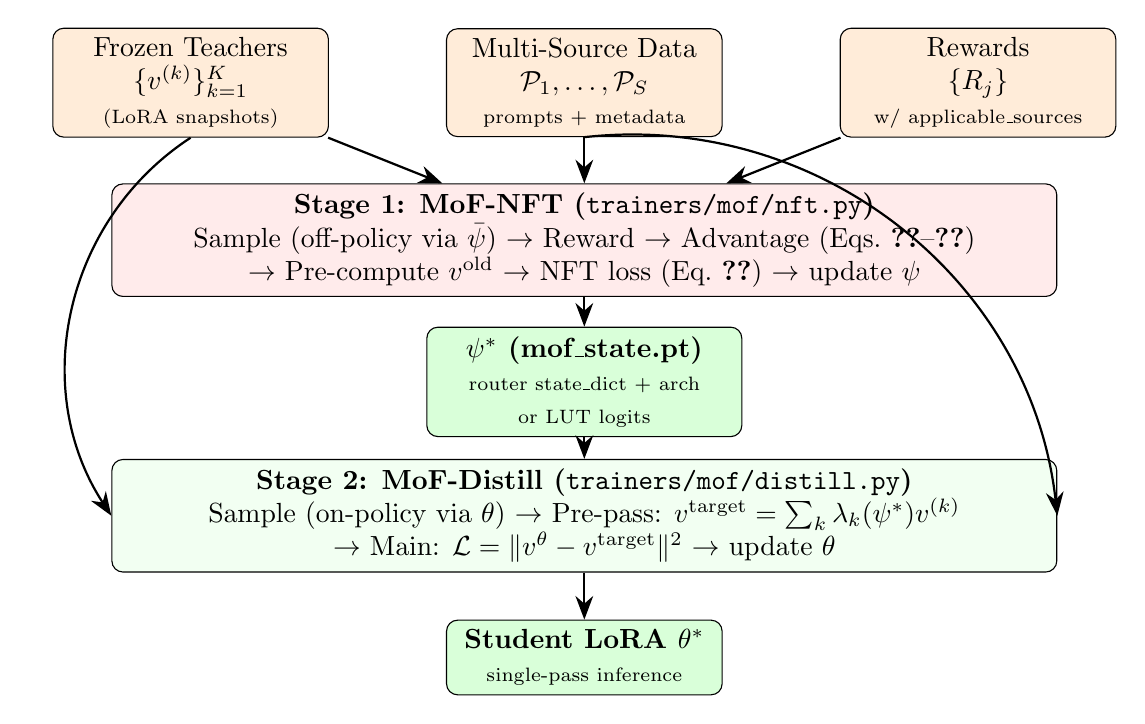
\begin{tikzpicture}[
    box/.style={draw, rounded corners, minimum width=4cm, minimum height=1cm, align=center, fill=blue!8},
    artifact/.style={draw, rounded corners, minimum width=3.5cm, minimum height=0.8cm, align=center, fill=orange!15},
    output/.style={draw, rounded corners, minimum width=3.5cm, minimum height=0.8cm, align=center, fill=green!15},
    arr/.style={-{Stealth[length=3mm]}, thick},
]
    \node[artifact] (teachers) at (0, 8) {Frozen Teachers\\$\{v^{(k)}\}_{k=1}^K$\\{\scriptsize (LoRA snapshots)}};
    \node[artifact] (data) at (5, 8) {Multi-Source Data\\$\mathcal{P}_1, \ldots, \mathcal{P}_S$\\{\scriptsize prompts + metadata}};
    \node[artifact] (rewards) at (10, 8) {Rewards\\$\{R_j\}$\\{\scriptsize w/ applicable\_sources}};

    \node[box, fill=red!8, minimum width=12cm] (stage1) at (5, 6) {
        \textbf{Stage 1: MoF-NFT (\texttt{trainers/mof/nft.py})}\\
        Sample (off-policy via $\bar\psi$) $\to$ Reward $\to$ Advantage (Eqs.~\ref{eq:step1}--\ref{eq:step3})\\
        $\to$ Pre-compute $v^{\text{old}}$ $\to$ NFT loss (Eq.~\ref{eq:nft_loss_full}) $\to$ update $\psi$
    };

    \node[output, minimum width=4cm] (psi) at (5, 4.2) {\textbf{$\psi^*$ (mof\_state.pt)}\\{\scriptsize router state\_dict + arch}\\{\scriptsize or LUT logits}};

    \node[box, fill=green!5, minimum width=12cm] (stage2) at (5, 2.5) {
        \textbf{Stage 2: MoF-Distill (\texttt{trainers/mof/distill.py})}\\
        Sample (on-policy via $\theta$) $\to$ Pre-pass: $v^{\text{target}}=\sum_k\lambda_k(\psi^*)v^{(k)}$\\
        $\to$ Main: $\loss = \|v^\theta - v^{\text{target}}\|^2$ $\to$ update $\theta$
    };

    \node[output] (theta) at (5, 0.7) {\textbf{Student LoRA $\theta^*$}\\{\scriptsize single-pass inference}};

    \draw[arr] (teachers) -- (stage1);
    \draw[arr] (data) -- (stage1);
    \draw[arr] (rewards) -- (stage1);
    \draw[arr] (stage1) -- (psi);
    \draw[arr] (psi) -- (stage2);
    \draw[arr] (teachers.south) to[bend right=45] (stage2.west);
    \draw[arr] (data.south) to[bend left=45] (stage2.east);
    \draw[arr] (stage2) -- (theta);
\end{tikzpicture}
\end{center}

\subsection{统一伪代码}

\begin{algorithm}[H]
\caption{End-to-End MoF Two-Stage Pipeline}
\label{alg:e2e}
\begin{algorithmic}[1]
\Statex \textbf{Input:} Frozen teachers $\{v^{(k)}\}$, sources $\{\mathcal{P}_s\}$, rewards $\{R_j\}$, base model $v^{\text{base}}$
\Statex \textbf{Output:} Student LoRA $\theta^*$ that approximates $v^{\MoF^*}$
\Statex
\State \textcolor{blue}{\textit{// =========== Stage 1: Train router $\psi$ ===========}}
\State Initialize $\psi$ (zeros / teacher\_biased / random); EMA $\bar\psi \gets \psi$
\For{epoch $= 1, \ldots, N_{\text{epochs}}^{(1)}$}
  \State samples $\gets$ \Call{Sample}{} \Comment{Alg.~\ref{alg:sample}, uses $\bar\psi$}
  \State $\{R_j(x_b)\}, \{\adv_b\} \gets$ \Call{ComputeRewardsAndAdvantages}{samples}
    \Comment{Eqs.~\ref{eq:step1}--\ref{eq:step3}}
  \State \Call{NFTOptimize}{samples, $\psi, \bar\psi$} \Comment{Alg.~\ref{alg:nft}}
  \State $\bar\psi \gets$ \Call{EMAStep}{$\psi$}
\EndFor
\State $\psi^* \gets \bar\psi$ (recommended) or $\psi$
\State Save $\psi^*$ + teacher\_names + router\_arch $\to$ \texttt{mof\_state.pt}

\Statex
\State \textcolor{blue}{\textit{// =========== Stage 2: Distill into student $\theta$ ===========}}
\State Load $\psi^*$ from \texttt{mof\_state.pt}; freeze $\psi^*$
\State Verify teacher snapshots (\texttt{\_verify\_teacher\_snapshots})
\State Initialize student $\theta$ (zeros LoRA on top of base)
\For{epoch $= 1, \ldots, N_{\text{epochs}}^{(2)}$}
  \State samples $\gets$ \Call{StudentSample}{} \Comment{Alg.~\ref{alg:distill_sample}}
  \State \Call{DistillOptimize}{samples, $\theta, \psi^*$} \Comment{Alg.~\ref{alg:distill}}
\EndFor
\State \Return $\theta^*$
\end{algorithmic}
\end{algorithm}

\subsection{部署期推理}

\begin{tcolorbox}[colback=green!5,colframe=green!50!black,title=\textbf{部署推理（Stage 2 完成后）}]
\begin{align}
x_T &\sim \N(0, I) \\
\text{for } i &= 0, \ldots, T-1: \\
&\quad v_i = v^{\theta^*}(x_{t_i}, t_i, c) \quad\textbf{(单次 forward,
\emph{不再}需要 router / teachers)}\\
&\quad x_{t_{i+1}} = \texttt{scheduler.step}(x_{t_i}, v_i, t_i)
\end{align}
\textbf{推理代价}：与单 LoRA 推理相同，相比 Stage 1 的
$K$-teacher + router forward，节省 $\sim K\times$ FLOPs。
\end{tcolorbox}

%% ============================================================
\section{代码 $\Leftrightarrow$ 公式对照表}
\label{sec:code_map}
%% ============================================================

\begin{center}
\renewcommand{\arraystretch}{1.4}
\footnotesize
\begin{tabular}{@{}p{6.5cm} l p{4cm}@{}}
\toprule
\textbf{公式 / 概念} & \textbf{文件} & \textbf{函数 / 行号} \\
\midrule
$x_{t_i} = (1-\sigma_i)x_0 + \sigma_i \varepsilon_i$ Eq.~\eqref{eq:flow_match_noise}
  & \texttt{nft.py} & \texttt{optimize}, Phase 1 (line $\sim$150) \\
$\mathcal{M}(v) = \|x_0^{\text{pred}}{-}x_0\|^2/w$ Eq.~\eqref{eq:self_norm_mse}
  & \texttt{nft.py} & \texttt{\_nft\_weighted\_mse} \\
$v^\pm$ Eqs.~\eqref{eq:v_plus}, \eqref{eq:v_minus}
  & \texttt{nft.py} & \texttt{optimize}, Phase 2 \\
$r = \mathrm{clamp}(\adv/(2A_{\max}){+}0.5, 0, 1)$ Eq.~\eqref{eq:r_def}
  & \texttt{nft.py} & \texttt{optimize}, Phase 2 \\
NFT total loss Eq.~\eqref{eq:nft_loss_full}
  & \texttt{nft.py} & \texttt{policy\_loss} computation \\
\midrule
3-step advantage Eqs.~\eqref{eq:step1}--\eqref{eq:step3}
  & \texttt{common.py} & \texttt{prepare\_feedback} \\
Per-set combined velocity (LUT) Eq.~\eqref{eq:per_sample_combined}
  & \texttt{common.py} & \texttt{\_combine\_velocities\_per\_sample} \\
Per-set combined velocity (router)
  & \texttt{common.py} & \texttt{\_compute\_combined\_velocity} \\
Sampling with $\sum_k \lambda_k v^{(k)}$
  & \texttt{common.py} & \texttt{\_mof\_inference\_context} \\
EMA off-policy split
  & \texttt{common.py} & \texttt{sampling\_context} \\
Safe teacher forward Alg.~\ref{alg:teacher_forward}
  & \texttt{common.py} & \texttt{\_compute\_teacher\_velocities} \\
\midrule
Router-induced teacher Eq.~\eqref{eq:router_teacher}
  & \texttt{distill.py} & \texttt{\_combine\_weighted} \\
Distill loss Eq.~\eqref{eq:distill_loss}
  & \texttt{distill.py} & \texttt{optimize}, main pass \\
2-pass design \S\ref{subsec:why_two_pass}
  & \texttt{distill.py} & \texttt{optimize} \\
Checkpoint validation \S 5.8
  & \texttt{distill.py} & \texttt{\_load\_mof\_weights}, \texttt{\_verify\_teacher\_snapshots} \\
LUT index semantics
  & \texttt{distill.py} & \texttt{\_get\_mof\_weights} (docstring) \\
\midrule
adaLN router architecture
  & \texttt{common.py} & \texttt{MoFAdaLNRouter} \\
LUT (K, T, S) module
  & \texttt{common.py} & \texttt{MoFMixingModule} \\
Bypass DDP for weight swap
  & \texttt{utils.py} & \texttt{bypass\_ddp\_for\_weight\_swap} \\
\bottomrule
\end{tabular}
\end{center}

%% ============================================================
\section{讨论}
\label{sec:discussion}
%% ============================================================

\subsection{Stage 1 与 Stage 2 的训练成本对比}

\paragraph{Stage 1 (NFT).} 每个 epoch：
\begin{itemize}[leftmargin=1.5em]
\item \textbf{Sample}: $K$ teacher forwards $\times$ $T$ timesteps $\times$ \texttt{num\_batches\_per\_epoch}
\item \textbf{Optimize}: $K$ teacher forwards $\times$ $T$ timesteps $\times$ $N_{\text{inner}}$
  (Phase 1, no\_grad) + $T$ student-style forwards with grad (Phase 2)
\end{itemize}
Reward evaluation 是额外开销（每个 sample 跑 $|\mathcal{R}|$ 个 reward
model）。可学习参数 $\sim 10^2$--$10^6$，optimizer state 极小。

\paragraph{Stage 2 (Distill).} 每个 epoch：
\begin{itemize}[leftmargin=1.5em]
\item \textbf{Sample}: $T$ student forwards（生成 trajectory）
\item \textbf{Optimize}: $K$ teacher forwards (pre-pass) + 1 student forward (main pass) per timestep $\times N_{\text{inner}}$
\end{itemize}
没有 reward 评估开销，loss 计算便宜（一个 MSE）。可学习参数 $\sim 10^7$
（LoRA），optimizer state 显著（AdamW 需要 2$\times$ 参数量的 momentum）。

\subsection{常见误区}

\begin{enumerate}[leftmargin=1.5em]
\item \textbf{把 Stage 2 的 trajectory 用在 Stage 1 上}：Stage 1 的
  \texttt{noised\_latents} 来自\emph{重新采样的高斯噪声}对 $x_0$ 加噪
  （Eq.~\eqref{eq:flow_match_noise}），\textbf{不是}走过的 trajectory 点。
  这是 NFT 与 GRPO 的本质差异——NFT 是 flow-matching MSE 风格，
  GRPO 才是 trajectory log-prob ratio 风格。
\item \textbf{把 Stage 1 的 sampling EMA 用在 Stage 2 上}：Stage 2 的
  $\psi^*$ 是\textbf{完全 frozen}的，没有 EMA／on-policy／off-policy
  概念。Student $\theta$ 自己决定 trajectory 分布（on-policy distillation）。
\item \textbf{在 Stage 2 重做 advantage}：Stage 2 没有 advantage / reward
  概念，它就是监督式 distillation。
\item \textbf{LUT 模式下用归一化 timestep 索引}：必须用 loop 计数器
  \texttt{timestep\_index}（0..$T{-}1$）查 LUT 列；用
  \texttt{t/1000} 会反向（最噪 step 取到最干净 step 的列）。
\end{enumerate}

\subsection{何时需要其他变体}

\begin{itemize}[leftmargin=1.5em]
\item \textbf{Stage 1 用 GRPO 而非 NFT}（\texttt{trainers/mof/grpo.py}）：
  当 dynamics 是 stochastic（CPS / Flow-SDE）且想用 importance ratio
  做 trust region 控制时。Stage 2 不变。
\item \textbf{Stage 2 加 KL penalty}：在 \eqref{eq:distill_total} 上叠加
  $\|v^\theta - v^{\text{ref}}\|^2$ 防止 student 偏离 base model 太远，
  类似 RLHF 中的 KL 锚定。
\item \textbf{多阶段迭代}：Stage 2 完成后把 $\theta^*$ 作为 base，重新跑
  Stage 1 训练一组新的 $\psi$（更精细的混合），再 Stage 2 蒸馏——
  渐进式 reward 改进。
\end{itemize}

\subsection{失败模式与排查}

\begin{center}
\renewcommand{\arraystretch}{1.4}
\footnotesize
\begin{tabular}{@{}p{4.5cm} p{5cm} p{4cm}@{}}
\toprule
\textbf{现象} & \textbf{可能原因} & \textbf{排查} \\
\midrule
所有 teacher 输出相同 & autocast cache 或 DDP buffer 未 bypass
& 检查 weight swap 循环外是否 disable autocast cache + bypass DDP \\
Stage 2 grad 极小 & 不会发生（model weight 空间无 mean-subtraction 瓶颈）
& 若发生，检查 $v^{\text{target}}$ 是否真的 detach；teacher snapshots 是否退化 \\
Stage 1 grad $\sim 10^{-10}$ & LoRA-shared-base 下 normalized-mixing 固有瓶颈
& 见 \texttt{mof\_per\_set\_analysis.tex} 第 14 节，考虑切换 Solution A (Direct Reward) \\
LUT distill 错位 & 用 \texttt{t/1000} 而非 loop counter 索引 LUT
& 检查 \texttt{\_get\_mof\_weights} 的 \texttt{timestep\_index} 来源 \\
Teacher snapshot 与 student 等同 & LoRA 加载失败（路径错 / 权重格式错）
& \texttt{\_verify\_teacher\_snapshots} 启动时报告 \\
Stage 2 reward 不如 Stage 1 & Distillation gap (student 容量不足 / 训练不充分)
& 增加 epoch；检查 student LoRA rank \\
\bottomrule
\end{tabular}
\end{center}

%% ============================================================
\section{结论}
\label{sec:conclusion}
%% ============================================================

\begin{tcolorbox}[colback=yellow!5,colframe=yellow!60!black,title=\textbf{核心结论}]
\begin{enumerate}[leftmargin=1.5em]
\item \textbf{二阶段训练把 reward 优化与推理压缩解耦}：Stage 1 用极少的
  mixing 参数找出 reward-optimal 的 teacher 加权策略；Stage 2 用一个
  独立的 student LoRA 把这个策略蒸馏成单 forward 推理。
\item \textbf{Stage 1 (NFT) 数学本质}：reward-weighted self-normalized
  MSE on $x_0$ reconstruction，配合 EMA 实现 off-policy。$\beta$ 在
  梯度中精确消去，仅通过 self-norm weight 作二阶 magnitude 调制。
\item \textbf{Stage 2 (Distill) 数学本质}：on-policy student trajectory 上的
  vanilla velocity MSE，target 由 frozen $\psi^*$ 加权 $K$ 个 teacher
  得到（Eq.~\eqref{eq:router_teacher}）。
\item \textbf{两阶段共享的硬性约束}：teacher forward 必须搭配
  \texttt{set\_autocast\_cache\_enabled(False)} +
  \texttt{bypass\_ddp\_for\_weight\_swap}，否则所有 teacher 静默退化为
  同一输出。Stage 2 的 2-pass 设计就是为了把 teacher forward 隔离在
  \texttt{accelerator.accumulate} 之外，规避这一约束与 DDP gradient
  路径的冲突。
\item \textbf{Bridge 是单向的}：$\psi^*$ 在 Stage 2 中完全 frozen；Stage
  2 不引入 reward / advantage / EMA / on-off-policy 区分——一旦
  $\psi^*$ 给定，Stage 2 退化为标准的 supervised distillation。
\end{enumerate}
\end{tcolorbox}

\end{document}
